%%%%%%%%%%%%%%%%%%%%%%%%%%%%%%%%%%%%%%%%%%%%%%%%%%%%%%%%%%%%%%%%%%%%%%%%%%%%%%%%
%2345678901234567890123456789012345678901234567890123456789012345678901234567890
%        1         2         3         4         5         6         7         8

\documentclass[letterpaper, 10 pt, conference]{ieeeconf}  % Comment this line out
                                                          % if you need a4paper
%\documentclass[a4paper, 10pt, conference]{ieeeconf}      % Use this line for a4
                                                          % paper

\IEEEoverridecommandlockouts                              % This command is only
                                                          % needed if you want to
                                                          % use the \thanks command
\overrideIEEEmargins
% See the \addtolength command later in the file to balance the column lengths
% on the last page of the document

\usepackage[utf8]{inputenc}
\usepackage[T1]{fontenc}

% The following packages can be found on http:\\www.ctan.org
\usepackage{graphicx} % for pdf, bitmapped graphics files
%\usepackage{epsfig} % for postscript graphics files
%\usepackage{mathptmx} % assumes new font selection scheme installed
%\usepackage{mathptmx} % assumes new font selection scheme installed
\usepackage{amsmath} % assumes amsmath package installed
%\usepackage{amssymb}  % assumes amsmath package installed

\title{\LARGE \bf
Lab1: Building a Simulator
}

%\author{ \parbox{3 in}{\centering Huibert Kwakernaak*
%         \thanks{*Use the $\backslash$thanks command to put information here}\\
%         Faculty of Electrical Engineering, Mathematics and Computer Science\\
%         University of Twente\\
%         7500 AE Enschede, The Netherlands\\
%         {\tt\small h.kwakernaak@autsubmit.com}}
%         \hspace*{ 0.5 in}
%         \parbox{3 in}{ \centering Pradeep Misra**
%         \thanks{**The footnote marks may be inserted manually}\\
%        Department of Electrical Engineering \\
%         Wright State University\\
%         Dayton, OH 45435, USA\\
%         {\tt\small pmisra@cs.wright.edu}}
%}

\author{Yiwen(Robert) Wu\\\\https://github.com/Robert1124/cse460}


\begin{document}



\maketitle
\thispagestyle{empty}
\pagestyle{empty}

\section{Exercise 1}

In the pursuit of commanding a point robot to trace an elliptical path in a two-dimensional plane, a control policy \( u(t) \) was formulated. This policy is rooted in the parametric representation of an ellipse, traditionally given by:

\begin{align}
    x(t) &= a \cos(\omega t + \phi), \\
    y(t) &= b \sin(\omega t + \phi),
\end{align}

where \( a \) and \( b \) denote the semi-major and semi-minor axes of the ellipse, \( \omega \) is the angular velocity, and \( \phi \) is the phase offset. For an ellipse centered at the origin and aligned with the axes, \( \phi \) is taken to be zero.

To derive the control inputs, we consider the time derivative of the parametric equations, yielding the velocity components of the robot at any instant:

\begin{align}
    \frac{dx}{dt} &= -a \omega \sin(\omega t), \\
    \frac{dy}{dt} &= b \omega \cos(\omega t).
\end{align}

These derivatives reflect the instantaneous velocity vector \( u(t) \) required to maintain the elliptical trajectory. For the specific case of uniform motion along the ellipse, \( \omega \) is set to 1, simplifying the control policy to:

\begin{align}
    u_x(t) &= -a \sin(t), \\
    u_y(t) &= b \cos(t).
\end{align}

The negative sign in \( u_x \) ensures that the motion proceeds in the counterclockwise direction when viewed from the positive z-axis, aligning with the conventional orientation for positive rotation.

The simulation framework utilizes a discrete-time model with a time step \( \Delta t \), iterating over a complete period \( T_f = 2\pi \), corresponding to the fundamental period of the sine and cosine functions. The initial conditions place the robot at the rightmost extremity of the ellipse by offsetting the center's x-coordinate by the semi-major axis length, while the y-coordinate remains unchanged. Specifically, with the ellipse's center at \( (3, 2) \) and a semi-major axis of 2, the initial position is computed as:

\begin{equation}
    \mathbf{x}_0 = \begin{bmatrix}
        3 + a \\
        2
    \end{bmatrix} = \begin{bmatrix}
        5 \\
        2
    \end{bmatrix}.
\end{equation}

Through an iterative simulation, the robot's state is updated according to the control policy, accurately reflecting the velocity vectors that are tangential to the desired elliptical path at every time step. The resulting data points can be visualized to verify adherence to the elliptical trajectory.

\begin{figure}[htbp]
    \centering
    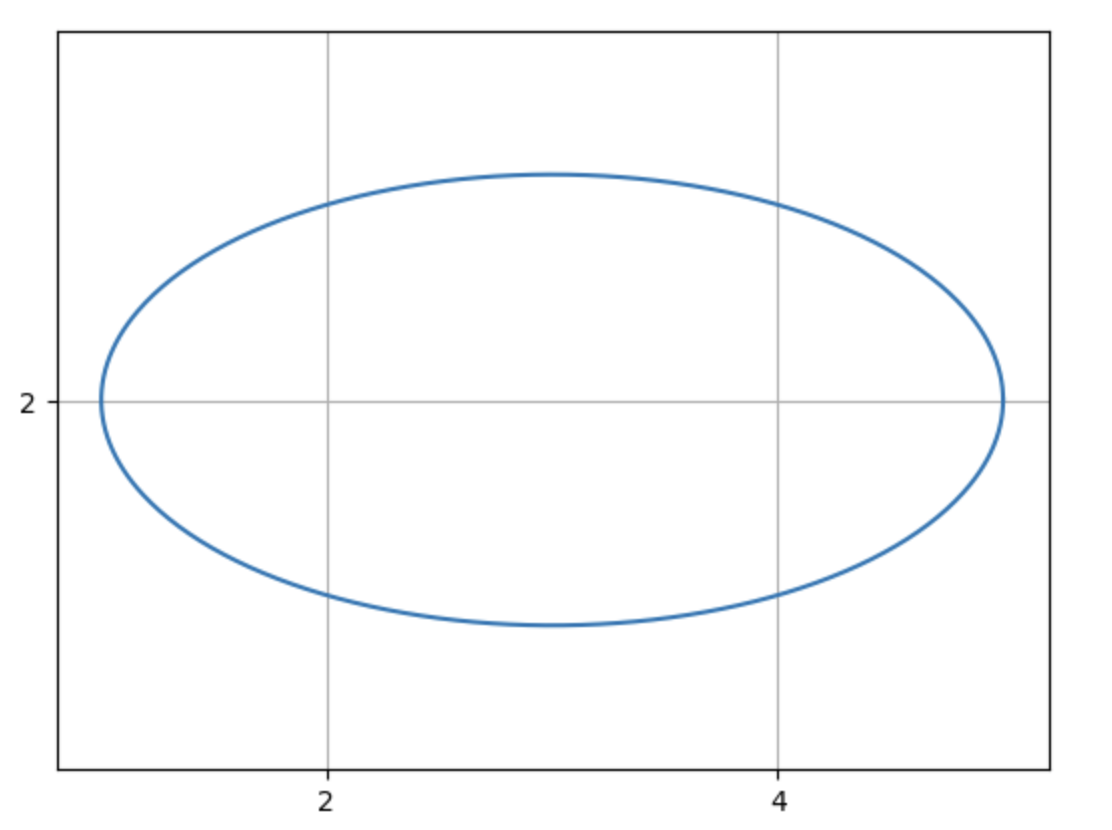
\includegraphics[width=0.5\textwidth]{image1.png}
\end{figure}

\section{Exercise 2}

To achieve the elliptical trajectory with a thirty-degree rotation, the control policy from the first exercise is modified. The modification involves rotating the control input velocity vector to align with the rotated ellipse.

A rotation matrix \( R \) is employed to transform the velocity vector. The matrix for a counterclockwise rotation by an angle \( \theta \) in 2D is given by:
\begin{equation}
    R(\theta) = \begin{bmatrix}
        \cos(\theta) & -\sin(\theta) \\
        \sin(\theta) & \cos(\theta)
    \end{bmatrix}
\end{equation}
This matrix is applied to the velocity vector \( \mathbf{u} = \begin{bmatrix} u_x \\ u_y \end{bmatrix} \) to obtain the rotated velocity vector.

The control policy function is defined as:
\begin{align}
    \text{control\_2}(t, y) &= \text{rotate}\left(\begin{bmatrix} -a \sin(t) \\ b \cos(t) \end{bmatrix}, \theta\right)
\end{align}
where \( a \) and \( b \) are the semi-major and semi-minor axes respectively, and \( \theta = \frac{\pi}{6} \) radians (30 degrees). The negative sign in the x-component ensures counterclockwise rotation.

For the initial conditions, the starting point on the ellipse must also be rotated. If the unrotated starting point is \( \mathbf{x}_0 \), the rotated initial position \( \mathbf{x} \) is obtained by:
\begin{equation}
    \mathbf{x} = \text{rotate}(\mathbf{x}_0 - \text{center}, \theta) + \text{center}
\end{equation}
where \textit{center} is the center of the ellipse.

The simulation proceeds by updating the robot's position using the rotated control inputs over the time interval \( [0, 2\pi] \) with a time step \( \Delta t = 0.01 \). This interval corresponds to one complete cycle of the elliptical path. The trajectory logged in \( \mathbf{x\_log} \) is expected to outline the rotated ellipse when plotted.

\begin{figure}[htbp]
    \centering
    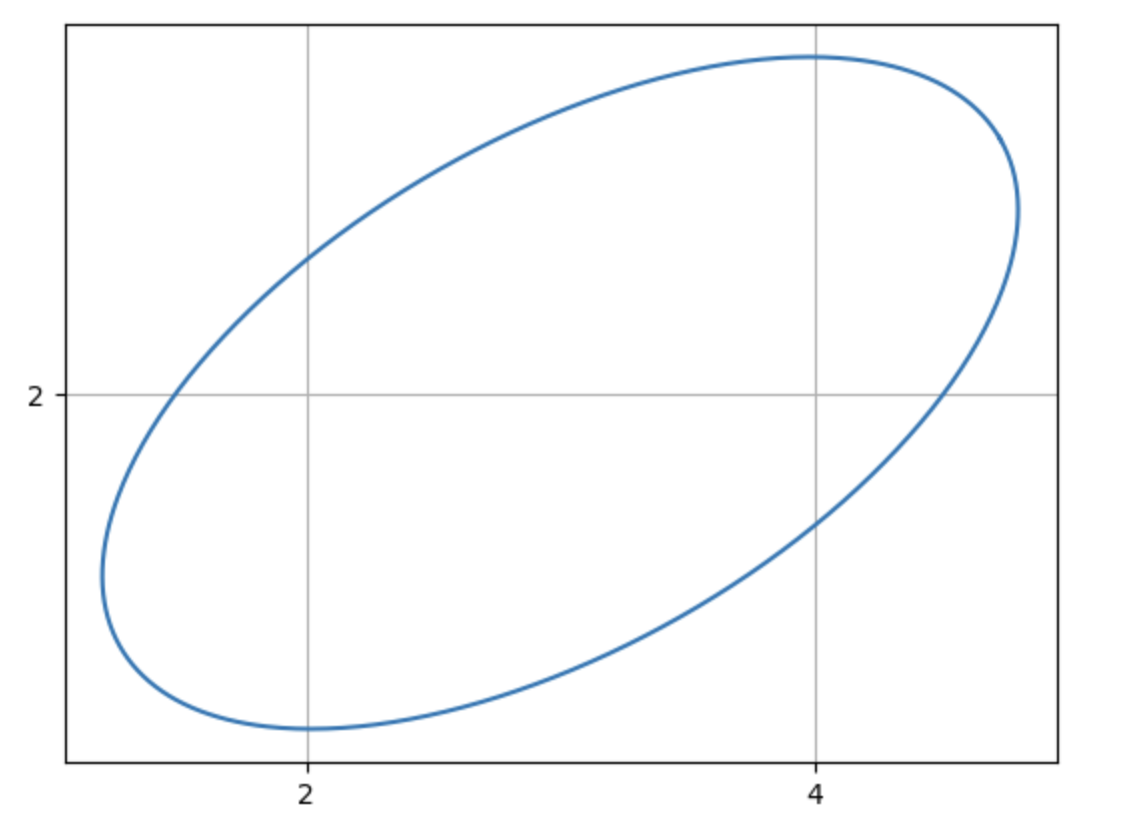
\includegraphics[width=0.5\textwidth]{image2.png}
\end{figure}

\section{Exercise 3}

The third exercise involves developing a control policy for a robot to follow the Lemniscate of Gerono, which is characterized by its figure-eight shape. The Lemniscate of Gerono can be described by parametric equations as follows:

\begin{align}
    x(t) &= a \cos(t), \\
    y(t) &= b \sin(2t),
\end{align}

where \( a \) and \( b \) are constants that scale the figure along the x and y axes respectively. To formulate the control inputs, the derivatives of these parametric equations are computed:

\begin{align}
    \frac{dx}{dt} &= -a \sin(t), \\
    \frac{dy}{dt} &= 2b \cos(2t).
\end{align}

The control inputs for the robot are the velocity components derived from these equations. The control policy function \textit{control\_3} is thus defined to return the velocity vector \( \mathbf{u} \):

\begin{equation}
    \mathbf{u}(t) = \begin{bmatrix}
        \frac{dx}{dt} \\
        \frac{dy}{dt}
    \end{bmatrix} = \begin{bmatrix}
        -a \sin(t) \\
        2b \cos(2t)
    \end{bmatrix}.
\end{equation}

A simulation loop is implemented to update the robot's position at discrete time intervals. The initial condition is set by evaluating the parametric equations at \( t = 0 \), thus starting the robot at one end of the figure-eight path. As time progresses, the control inputs guide the robot along the Lemniscate, and the resulting trajectory is logged in \( \mathbf{x\_log} \).

The complete trajectory is simulated over a time period \( T_f = 2\pi \) with a time step \( \Delta t = 0.01 \), ensuring that the robot completes the figure-eight pattern within the duration. The trajectory can be visualized by plotting \( \mathbf{x\_log} \), confirming the efficacy of the control policy in achieving the desired path.

\begin{figure}[htbp]
    \centering
    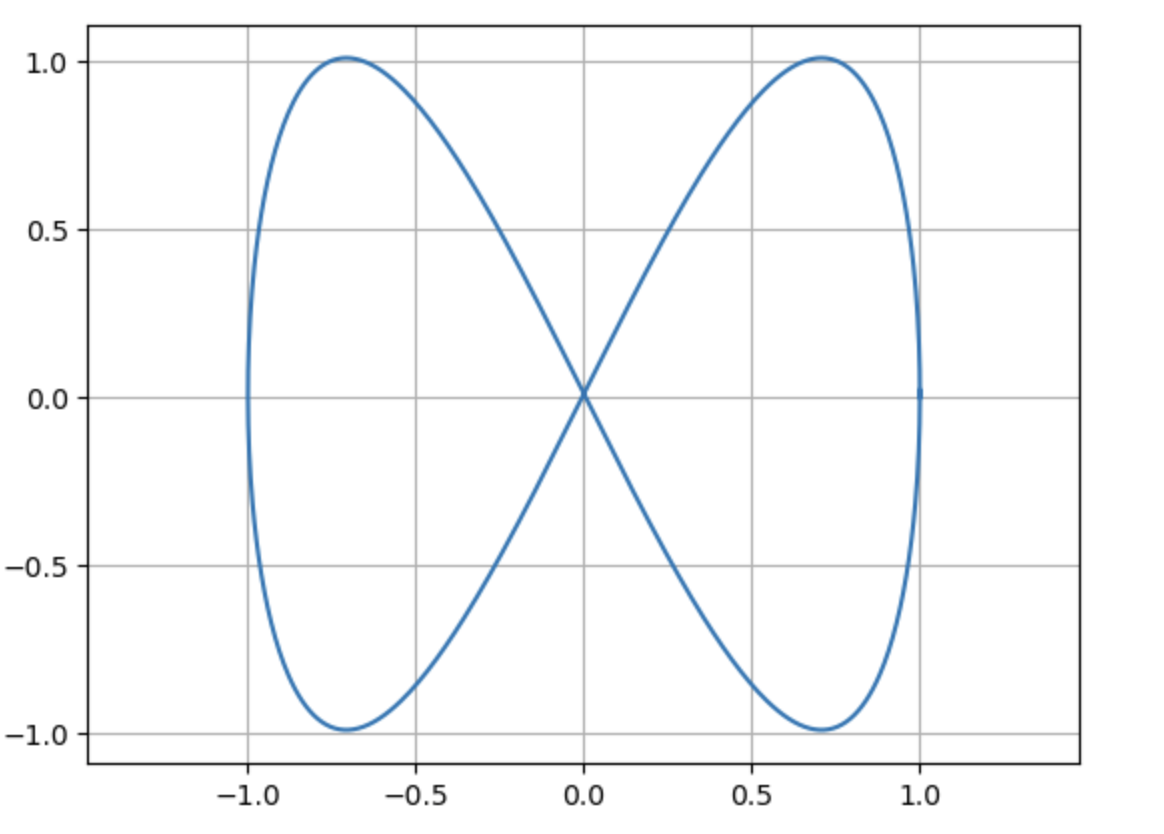
\includegraphics[width=0.5\textwidth]{image3.png}
\end{figure}

\section{Exercise 4}

The fourth exercise extends the simulation environment to include external disturbances in the form of wind while the robot is executing a circular trajectory. To accurately reflect these conditions, the \texttt{simulate} function is enhanced to integrate the effects of wind into the robot's dynamics.

\subsection*{Control Policy Function}
A control policy for circular motion, denoted as \texttt{control\_4}, is defined to produce control inputs \( u_x \) and \( u_y \) that adhere to the following equations:
\begin{align}
    u_x(t) &= -a \sin(t), \\
    u_y(t) &= a \cos(t),
\end{align}
where \( a \) represents the radius of the circular path.

\subsection*{Simulation Function with Wind}
The simulation function, named \texttt{simulate\_4}, accepts additional parameters for wind influence:
\begin{itemize}
    \item \texttt{wind\_constant} is a vector representing a constant wind force applied to the robot.
    \item \texttt{wind\_random\_std} is the standard deviation of a zero-mean Gaussian distribution from which random wind perturbations are sampled.
\end{itemize}

The state update equation, incorporating the wind components, is expressed as:
\begin{equation}
    \mathbf{x} \leftarrow \mathbf{x} + \Delta t (\mathbf{u} + \mathbf{w}_{\text{constant}} + \mathbf{w}_{\text{random}}),
\end{equation}
where \( \mathbf{w}_{\text{random}} \) is the random wind vector generated at each time step.

\subsection*{Simulation Execution}
Two simulations are conducted:

\begin{enumerate}
    \item The first simulation introduces a constant wind vector \( \mathbf{w}_{\text{constant}} = [0.1, 0.1]^\top \) throughout the robot's motion.
    \item The second simulation models wind as a random process with a standard deviation of \( \sigma_{\text{wind}} = 0.1 \), affecting the robot in both x and y directions independently.
\end{enumerate}

The robot's trajectory is recorded in two separate logs, \texttt{x\_log\_constant\_wind} and \texttt{x\_log\_random\_wind}, representing the path under constant and random wind conditions, respectively.

\begin{figure}[htbp]
    \centering
    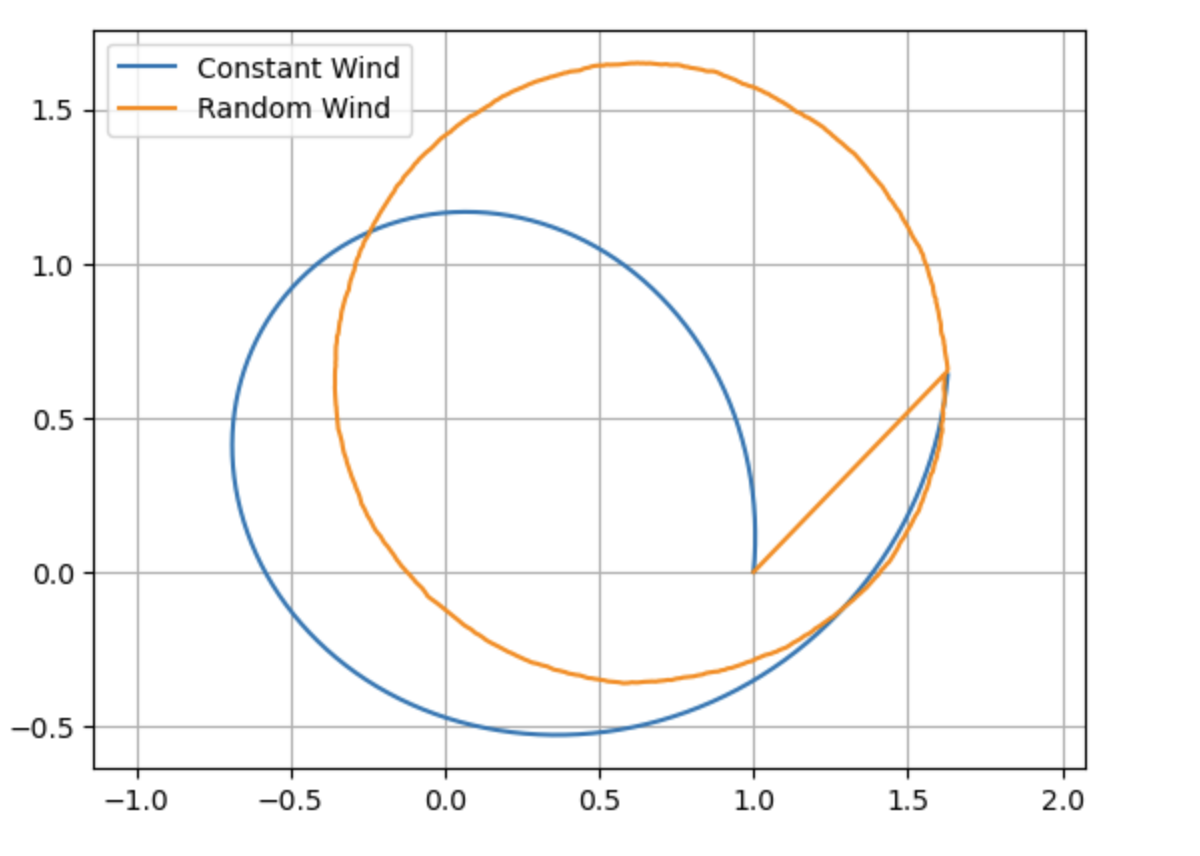
\includegraphics[width=0.5\textwidth]{image4.png}
\end{figure}

\end{document}
